\documentclass[border=10pt]{standalone}
\usepackage{tkz-euclide}

\usepackage{tikz}
\usetikzlibrary{calc,
                intersections,
                arrows.meta
                }

\begin{document}

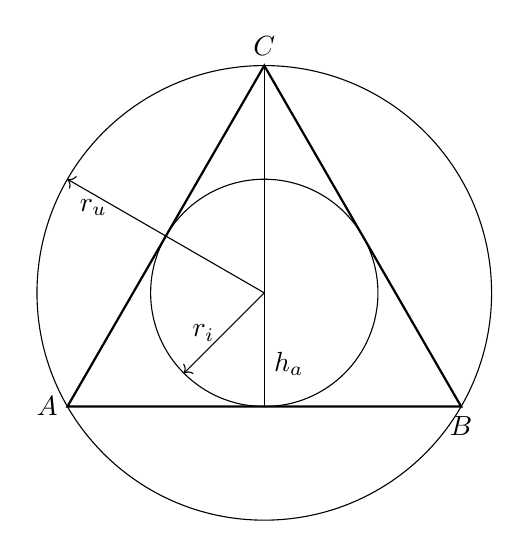
\begin{tikzpicture}
    % Koordinaten der Eckpunkte des Dreiecks
    \coordinate [label=left:$A$] (A) at (0,0);
    \coordinate [label=below:$B$] (B) at (5,0);
    \coordinate [label=above:$C$] (C) at (2.5,4.33);

    % Zeichne das Dreieck
    \draw[thick] (A) -- (B) -- (C) -- cycle;

    % Zeichne Höhe auf a
    \coordinate (fpha) at ($(A)!(C)!(B)$); % Fusspunkt Höhe a
    \draw (fpha) -- node[right, very near start] {$h_a$} (C);

    % Berchne Inkreisradius
    \pgfmathsetmacro{\ri}{5/(2*3^(1/2))}

    % Zeichne Inkreis
    \coordinate (mpik) at ($(fpha)+(0,\ri)$); % Mittelpunkt Inkreis
    \draw (mpik) circle [radius=\ri];

    % Zeichne Inkreisradius
    \def\angle{225};
    \draw[->] (mpik) -- node[left] {$r_i$} +({\angle}:\ri);
    
    % Berechne Umkreisradius
    \pgfmathsetmacro{\ru}{5/(3^(1/2))};

    % Zeichne Umkreis
    \draw (mpik) circle [radius=\ru];

    % Zeichne Umkreisradius
    \draw[->] (mpik) -- node[left, near end] {$r_u$} (90:\ru);

    % Berechne Seitenlängen
    \pgfmathsetmacro{\a}{8^(1/2)}
    \pgfmathsetmacro{\b}{13^(1/2)}
    \pgfmathsetmacro{\c}{5}

    
\end{tikzpicture}

\end{document}